% This is a LaTeX template kindly taken from Jernej Debevec.
% Provided by Miha Muskinja for the purpose of the seminar I in the 1st year
% of the 2nd cycle of the study of physics at the Faculty of Mathematics and Physics, University of Ljubljana.

% Set the document class and options
\documentclass[10pt, titlepage, a4paper]{article}
\usepackage[a4paper, inner=2.5cm, outer=2.5cm, top=2.25cm, bottom=2.25cm]{geometry}
\usepackage{graphicx}
\usepackage{hyperref}
\usepackage{wrapfig}
\usepackage{float}
\usepackage{amsmath}
\usepackage{amssymb}
\usepackage{amsfonts}
\usepackage{bm}
\usepackage{dirtytalk}
\usepackage{cleveref}
\hypersetup{colorlinks=true}

% Load the natbib package for citation style
\usepackage{natbib}

% Some macros for commonly used symbols in physics/quantum mechanics
\newcommand{\bb}[1]{\bm#1}
\newcommand{\dd}{\mathrm{d}}
\newcommand{\pp}{\partial}
\newcommand{\dg}{\dagger}
\newcommand{\la}{\langle}
\newcommand{\ra}{\rangle}
\newcommand{\id}{\mathbb{1}}
\newcommand{\T}{\mathsf{T}}
\newcommand{\ua}{\uparrow\>}
\newcommand{\da}{\downarrow\>}
\newcommand{\fs}[1]{\slashed{#1}}  % Feynmann slash
\newcommand{\mc}[1]{\mathcal{#1}}
\newcommand\thickbar[1]{\accentset{\rule{.5em}{.03em}}{#1}}
\renewcommand{\bar}{\thickbar}

% Start the document
\begin{document}

% The title page
\begin{titlepage}
{\centering

\includegraphics[width=6cm]{logo_fmf.pdf}

\vspace{0.8cm}
{\small Department of Physics}

\vspace{5cm}
\vspace{0.5cm}
{\huge\textbf{Distribution of Data Transmission in a}} \\
\vspace{0.2cm}
{\huge\textbf{Randomized Computer Network}} \\
\vspace{0.5cm}
{\large\textbf{Final Assignment for Model Analysis 1, 2023/24}}

\vfill
\textbf{Author:} Marko Urbanč \\
\textbf{Professor:} Prof. Dr. Simon Širca \\ 
\textbf{Advisor:}  doc. dr. Miha Mihovilovič \\

\vspace{1cm}
Ljubljana, August 2024 \\
}
\vspace{3cm}
\end{titlepage}

% Add table of conents
\hypersetup{pageanchor=true}
\pagenumbering{roman}
\setcounter{page}{2}
\tableofcontents
\vspace{1cm}

% Proceed with the main body
\pagenumbering{arabic}

% Sections based on typical Model Analysis structure
\section{Introduction}
The scope of computer networks has been expanding rapidly in the past few decades. What once were simple 
networks of interconnected computers have now evolved into complex systems that are used for a wide range of
applications. It makes sense then for one to plan and analyze the flow of data in such networks to ensure that
they are efficient and reliable and thus cheaper to maintain. \\

As my final assignment for Model Analysis 1, I opted to simulate the flow of data in a randomized computer network. The network 
consists of a $N\times N$ grid, where each unit of the grid can be a server, a user or a wire used to connect the two. Each of these 
units is connected to its four nearest neighbors and has a value associated with it that specifies it's bandwidth. For wires this is the 
maximum data throughput, for servers it is the maximum data processing rate and for users it is the maximum data consumption rate. We'd like 
to find the distribution of server-loads for a grid of wires with random bandwidths. It is possible to study many different types of 
server and user placements but the most interesting one to us will be where we have the users and servers placed on the top and bottom 
rows of the grid, respectively. \\

We can solve for the flow rates through the network by solving a set of constrained linear equations. This field of study is
known as linear programming and is a powerful tool for solving optimization problems. We've already seen some linear programming 
use in the second task of this course \texttt{mod102} where we created a dietary plan from a set of given foods based on their costs 
and nutritional values. For the sake of completeness it makes sense to quickly go over the basics of linear programming before we
proceed with the simulation. Linear programming uses linear optimization to find the maximum or minimum of a linear function
subject to a set of linear constraints. This function is known as the objective function and is quite analogous to the cost 
function we've seen mentioned in the world of Machine Learning. The constraints are linear inequalities or equations that
define the feasible region of the problem. Mathematically formulated we can consider a cost function $f(x)$ and a set of 
constraints defined as:
%
\begin{gather*}
    f(x_1, x_2, \dots, x_n) = c_1x_1 + c_2x_2 + \dots + c_nx_n\>, \\
    a_{11}x_1 + a_{12}x_2 + \dots + a_{1n}x_n \leq b_1\>, \\
    a_{21}x_1 + a_{22}x_2 + \dots + a_{2n}x_n \leq b_2\>, \\
    \vdots \\
    a_{m1}x_1 + a_{m2}x_2 + \dots + a_{mn}x_n \leq b_m\>.
\end{gather*}
%
The goal is then to find the values of $x_1, x_2, \dots, x_n$ that maximize or minimize the cost function $f(x)$ while satisfying
the constraints. The feasible region is the set of all points that satisfy the constraints and the optimal solution is the point in
the feasible region that maximizes or minimizes the cost function. That is all that is necessary from a mathematical perspective. Of course 
the actual implementation of solvers for such problems are much more complex and involve a lot of optimization techniques but that is 
not the focus of this assignment. \\

\section{Task}
The original text of the assignment reads as follows:
\begin{quote}
    \centering
    \textbf{Razporejanje prenosa podatkov po omrežju:} Za model omrežja vzemi $N\times N$ kvadratno mrežo, vsak rob pa ima naključno 
    maksimalno hitrost povezave med $0$ in $1$. Vozlišča na zgornjem robu so internetni odjemalci, spodnji rob pa so strežniki. V notranjih
    vozliščih velja 1. Kirchhoffov zakon. S pomočjo linearnega programiranja določi, kolikšne hitrosti prenosa imajo strežniki in odjemalci, 
    ko je skupna hitrost prenosa največja. Ker gre za naključna omrežja, si oglej tudi statistično porazdelitev zanimivih količin.
\end{quote}

Translated to English this reads:
\begin{quote}
    \centering
    \textbf{Distribution of Data Transmission in a Network:} Take a $N\times N$ square grid as the network model, where each edge has a random 
    maximum connection speed between $0$ and $1$. The nodes on the top edge are internet clients, while the bottom edge are servers. 
    In the internal nodes, Kirchhoff's first law holds. Using linear programming, determine the transmission speeds of the servers and clients 
    when the total transmission speed is maximized. Since these are random networks, also examine the statistical distribution of 
    interesting quantities.
\end{quote}

\section{Solution Overview}
I took upon the task of simulating the flow of data in Python using \texttt{PuLP} as my choice of linear programming library among others 
such as \texttt{numpy}, \texttt{scipy} and \texttt{matplotlib}. I'm aware that more complex network simulation packages exist for Python, 
such as \texttt{networkx}, but I wanted to keep the simulation as simple as possible and home-brewed. To start I created the base classes,
\texttt{User}, \texttt{Server} and \texttt{Wire} that represent the nodes of the network. Among other things each of these classes has a \texttt{bandwidth}
attribute that specifies the maximum data throughput, processing rate and consumption rate, respectively. The other attributes 
determine the position of the node in the grid, its ID etc. All these classes are slotted into a \texttt{Grid} class 
that represents the network as a whole. The \texttt{Grid} class contains the necessary methods to setup the network, 
solve the linear problem and extract or plot the results. \\

I think it makes sense to go over the various constraints I've imposed on the network. The most challenging part of setting 
the constraints was my want to use the absolute values of the flow rates in the linear equations. This becomes a problem 
because the absolute value function is not linear and thus not directly compatible with linear programming. To get around 
this I've used the following trick. I've introduced two new variables $\rho^+$ and $\rho^-$ that represent the positive and
negative parts of the flow rates, respectively. Both of these quantities are non-negative and their sum is equal to the
absolute value of the flow rate, such that $\rho = \rho^+ - \rho^-$. This way I can rewrite the absolute value of the flow rate
as a linear combination of $\rho^+$ and $\rho^-$. \\ 

The next step was to impose constraints for the flow rates through the 
network. The flow rates are determined by the bandwidths of the wires, servers and users. Wires are allowed to transmit 
data in both directions thus the absolute value of the flow rate cannot exceed two times the bandwidth of the wire. The sum 
of the flow rates into a Wire node must be equal to the sum of the flow rates out of the Wire. Servers and Users are special 
cases since they cause a divergence in what we could call the flow field, if we had a continuous field. The flow rate into a
Server is strictly zero (thus $\rho^- = 0$). Likewise the flow rate out of a User is also strictly zero. The maximum flow
rate into a User is determined by its bandwidth. The way I've set up the constraints is that the users demand the 
maximum amount of data they can consume unconditionally while the servers are allowed to process data at
a rate that is less than or equal to their bandwidth. \\

The objective function of the linear problem is to satisfy the demands of the users while minimizing the flow rates 
through the network and minimizing server loads. The flow rates are minimized by minimizing the sum of the positive and
negative parts of the flow rates. The server loads are minimized by minimizing the sum of the flow rates into the servers.
The objective function is thus a linear combination of the flow rates and server loads. \\

The way the problem has been set up results in two sets of data for flow rates, one for the positive part and
one for the negative part. The two are equal in magnitude but opposite in sign and we can consider the real 
solution to be one or the other. The flow rate divergence is thus given by the sum of the two. The term flow rate 
divergence is used here to describe data that is either consumed or produced by the network. The flow rate divergence
must thus be zero at all nodes except for the Users and Servers. \\

To stick with the purpose of having a home-brewed simulation I also drew some icons for the Users and Servers in a pixel 
art style. 

\section{Results}
\subsection{Basic Configuration}
First I ran the simulation for a $30\times 30$ grid with wires having bandwidths between $0$ and $1$. It is important to note 
that the bandwidths were not sampled uniformly but rather from a beta distribution. The beta distribution is a 
continuous probability distribution that is defined on the interval $[0, 1]$. It is a good choice for this problem
since we can easily skew the distribution towards the lower or higher bandwidths. Having a uniform distribution yielded 
grids that were infeasible to solve. The \textcolor{red}{\Cref{fig:beta_dist}} shows the probability density function
of the beta distribution for different values of the shape parameters $\alpha$ and $\beta$. The shape parameters determine
the skewness of the distribution. 

\begin{figure}[H]
    \centering
    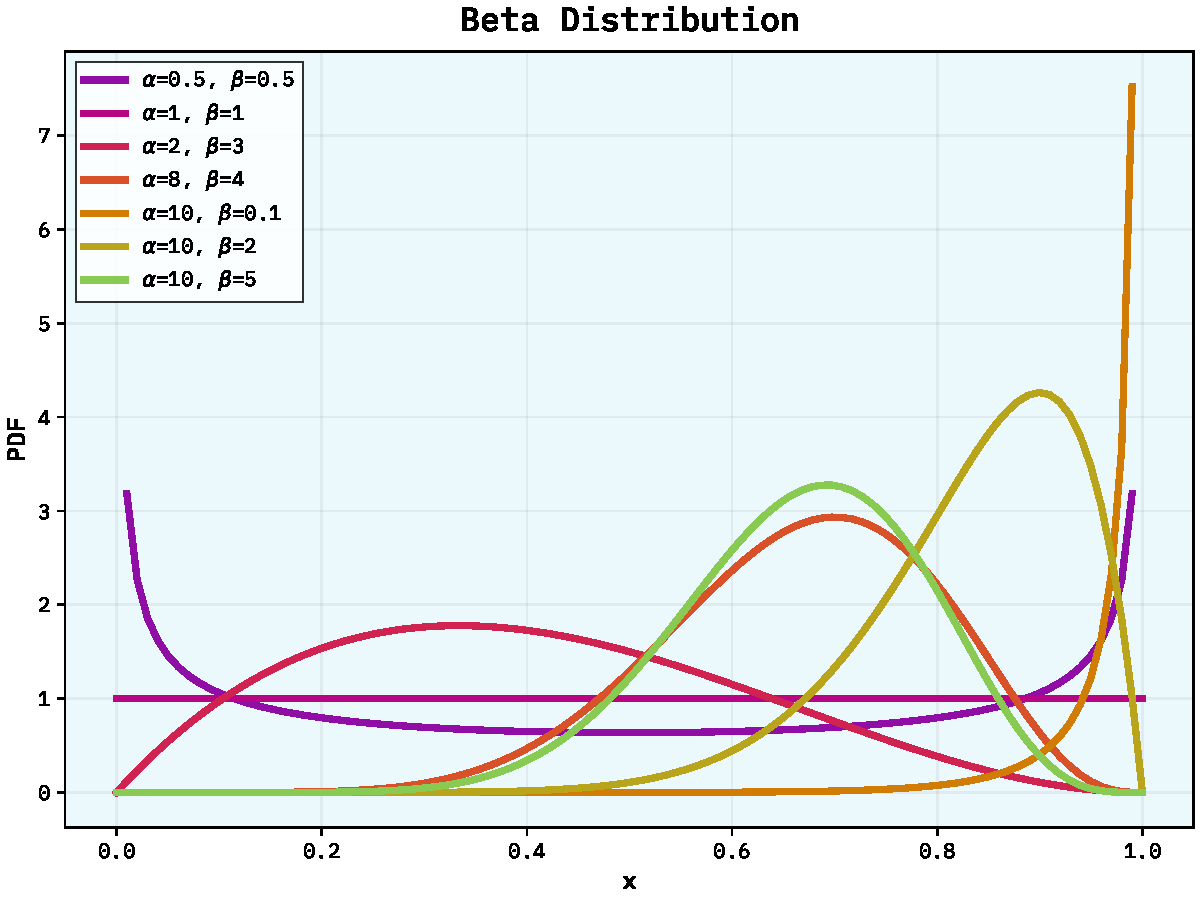
\includegraphics[width=0.8\textwidth]{../Images/beta_dist.pdf}
    \caption{Probability density function of the beta distribution for different values of the shape parameters $\alpha$ and $\beta$.}
    \label{fig:beta_dist}
\end{figure}

We can see the results of a basic simulation for a $10\times 10$ grid in \textcolor{red}{\Cref{fig:basic_grid}}. The wires 
in this grid have bandwidths sampled from a beta distribution with $\alpha = 10$ and $\beta = 2$. For illustrative purposes
I've colored the nodes based on their flow rate divergence and plotted both the positive and negative parts of the 
flow rates.

\begin{figure}[H]
    \centering
    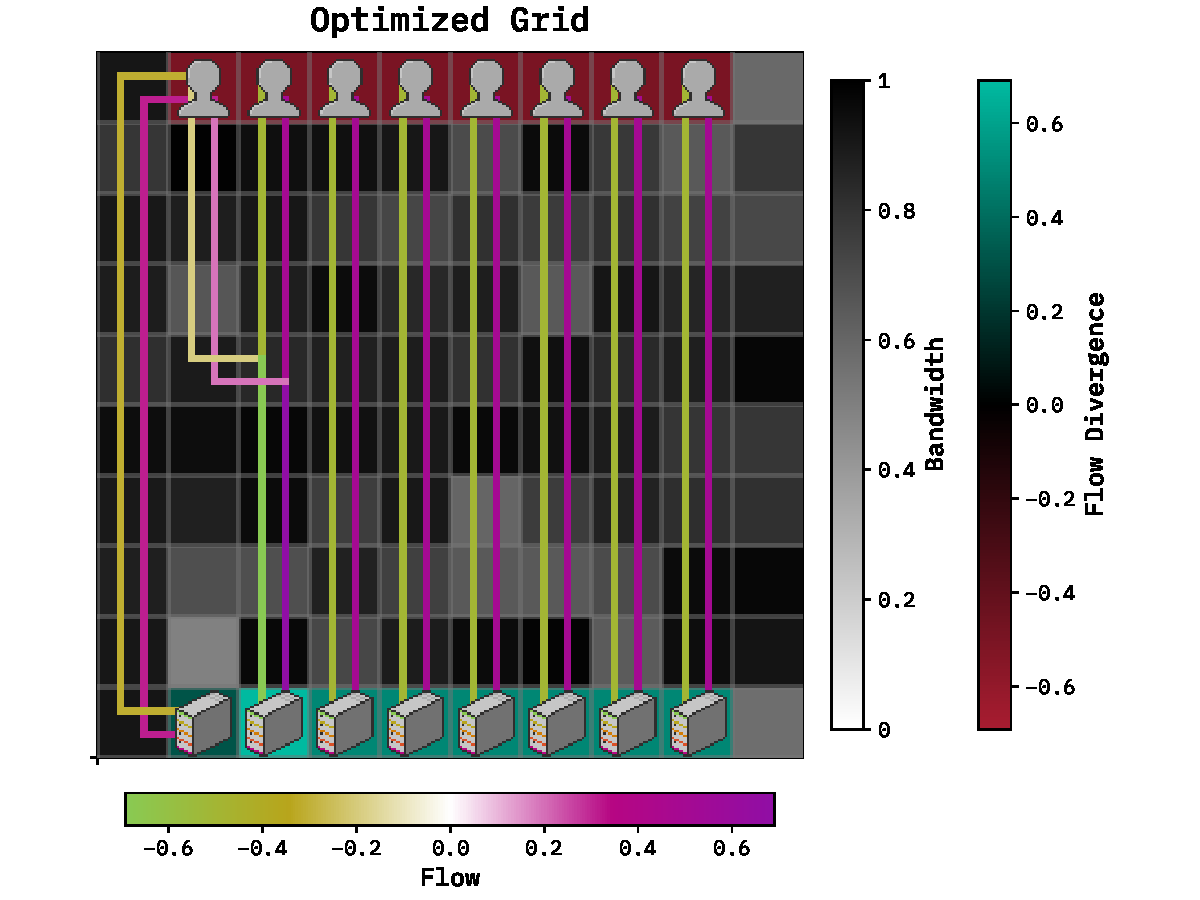
\includegraphics[width=0.92\textwidth]{../Images/optimize-case-10.pdf}
    \caption{Flow rate divergence in a $10\times 10$ grid with wires having bandwidths sampled from a beta distribution with $\alpha = 10$ and $\beta = 2$.}
    \label{fig:basic_grid}
\end{figure}

We can see that the flow rate divergence is zero at all nodes except for the Users and Servers. The flow of data goes almost 
as linearly as possible from the Users to the Servers, however due to the objective functions demand to minimize server loads 
the flow rates are not uniform. We can see on the left-hand side of the grid that the flow is higher for the second server and lower 
for the first. The first user receives data from both these servers as a portion of the data is carried over from the second 
server. This is likely due to wires in the direct path to the first server having lower bandwidths, thus making it cheaper 
to carry the data over from the second server and to place the original connection to the first user slightly to the side.


\section{Conclusion and Comments}

% Add references
% \newpage
% \bibliographystyle{unsrt}
% \bibliography{mod100}

% End document
\end{document}

